\documentclass[12pt]{book}
\usepackage[utf8]{inputenc}
\usepackage[paperwidth=6in, paperheight=9in]{geometry}
\usepackage{graphicx}
\usepackage{multicol}
\usepackage{enumitem}
\usepackage{ccicons}
\usepackage{url}
\usepackage{fmtcount}

%\pagestyle{headings}

% https://www.amazon.com/BookFactory%C2%AE-Password-Passwords-Notebook-JOU-120-MCW/dp/B009YK2GOA/ref=redir_mobile_desktop?ie=UTF8&ref_=aw_cm_cr_asin_lnk

%http://www.lulu.com/shop/wade-brainerd/password-logbook/hardcover/product-22927496.html

%gsort -R diceware.wordlist | head -n 4 | cut -f2 | tr -d '\n' | tee password | shasum

\begin{document}

\pagenumbering{gobble}

\newpage
\thispagestyle{empty}

%\noindent
%Owner \
%\vspace{-.1in} \\ \rule{\textwidth}{.2pt}
%\vspace{.5in}
%
%\noindent E-mail \
%\vspace{-.1in} \\ \rule{\textwidth}{.2pt}
%\vspace{.5in}
%
%\noindent Mobile phone \
%\vspace{-.1in} \\ \rule{\textwidth}{.2pt}
%\vspace{.5in}
%
%\noindent Home phone \
%\vspace{-.1in} \\ \rule{\textwidth}{.2pt}
%\vspace{.5in}
%
%\noindent Address \
%\vspace{-.1in} \\ \rule{\textwidth}{.2pt}
%
%\vspace{0.75in}

\vspace*{\fill}

If found, please return to:\vfill



\newpage

\chapter*{Record of Important Things}

\begin{center}
	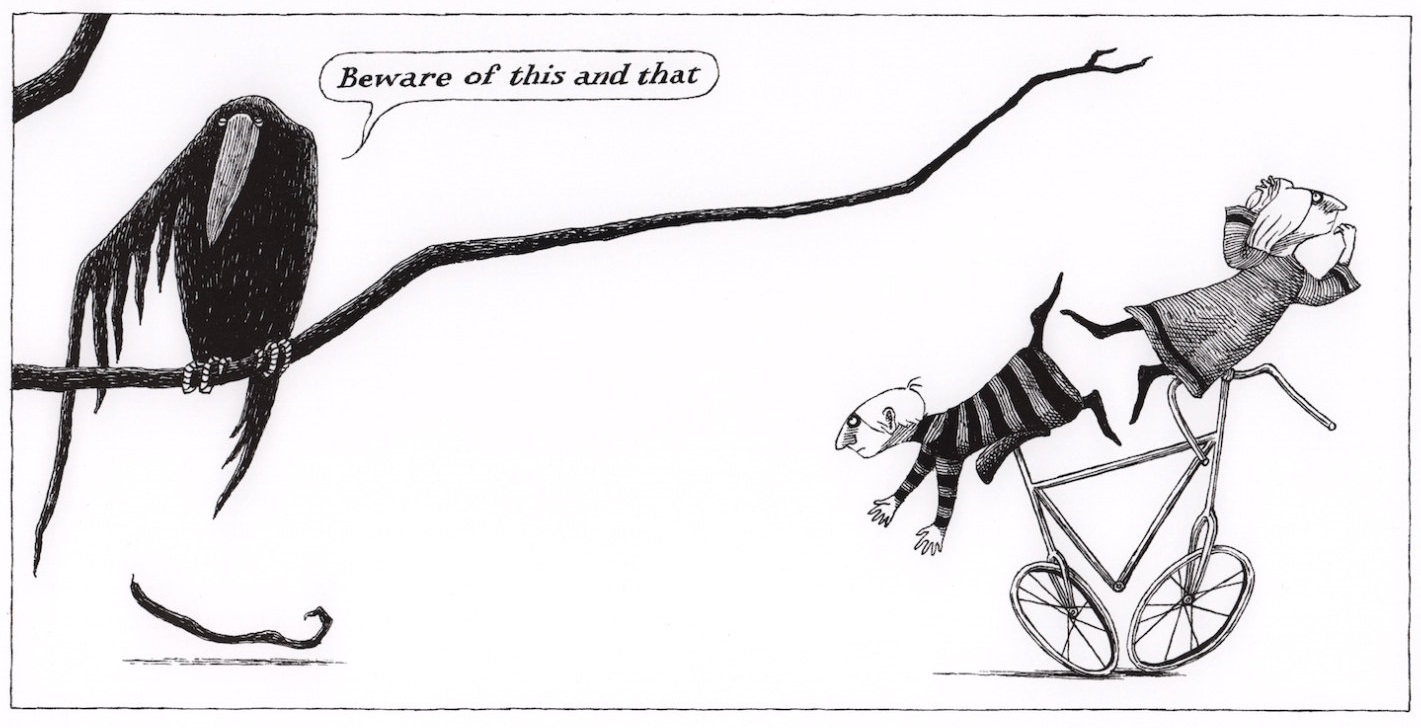
\includegraphics[width=\textwidth]{gorey.png}
\end{center}

\begin{small}
\textit{Simply, people can no longer remember passwords good enough to reliably defend against dictionary attacks, and are much more secure if they choose a password too complicated to remember and then write it down. We're all good at securing small pieces of paper. I recommend that people write their passwords down on a small piece of paper, and keep it with their other valuable small pieces of paper: in their wallet.}
\begin{flushright}{Bruce Schneier CTO, Resilient}\end{flushright}
\end{small}

\newpage
\thispagestyle{empty}

\begin{center}
{\large
Index \vspace{.5in}
}

\begin{tabular}{l l l l }
	1 & \multicolumn{3}{l}{Record of authentication credentials and other notes} \vspace{.225in} \\
	1 & \rule{1.75in}{.2pt} & 2 & \rule{1.75in}{.2pt} \vspace{.225in} \\
	3 & \rule{1.75in}{.2pt} & 4 & \rule{1.75in}{.2pt} \vspace{.225in} \\
	5 & \rule{1.75in}{.2pt} & 6 & \rule{1.75in}{.2pt} \vspace{.225in} \\
	7 & \rule{1.75in}{.2pt} & 8 & \rule{1.75in}{.2pt} \vspace{.225in} \\
	9 & \rule{1.75in}{.2pt} & 10 & \rule{1.75in}{.2pt} \vspace{.225in} \\
	11 & \rule{1.75in}{.2pt} & 12 & \rule{1.75in}{.2pt} \vspace{.225in} \\
	13 & \rule{1.75in}{.2pt} & 14 & \rule{1.75in}{.2pt} \vspace{.225in} \\
	15 & \rule{1.75in}{.2pt} & 16 & \rule{1.75in}{.2pt} \vspace{.225in} \\
	17 & \rule{1.75in}{.2pt} & 18 & \rule{1.75in}{.2pt} \vspace{.225in} \\
	19 & \rule{1.75in}{.2pt} & 20 & \rule{1.75in}{.2pt} \vspace{.225in} \\
	21 & \rule{1.75in}{.2pt} & 22 & \rule{1.75in}{.2pt} \vspace{.225in} \\
	23 & \rule{1.75in}{.2pt} & 24 & \rule{1.75in}{.2pt} \vspace{.225in} \\
\end{tabular}

\end{center}

\newpage
\thispagestyle{empty}

\begin{center}
	
\begin{tabular}{l l l l }
	25 & \rule{1.75in}{.2pt} & 26 & \rule{1.75in}{.2pt} \vspace{.225in} \\
	27 & \rule{1.75in}{.2pt} & 28 & \rule{1.75in}{.2pt} \vspace{.225in} \\
	29 & \rule{1.75in}{.2pt} & 30 & \rule{1.75in}{.2pt} \vspace{.225in} \\
	31 & \rule{1.75in}{.2pt} & 32 & \rule{1.75in}{.2pt} \vspace{.225in} \\
	33 & \rule{1.75in}{.2pt} & 34 & \rule{1.75in}{.2pt} \vspace{.225in} \\
	35 & \rule{1.75in}{.2pt} & 36 & \rule{1.75in}{.2pt} \vspace{.225in} \\
	37 & \rule{1.75in}{.2pt} & 38 & \rule{1.75in}{.2pt} \vspace{.225in} \\
	39 & \rule{1.75in}{.2pt} & 40 & \rule{1.75in}{.2pt} \vspace{.225in} \\
	41 & \rule{1.75in}{.2pt} & 42 & \rule{1.75in}{.2pt} \vspace{.225in} \\
	43 & \rule{1.75in}{.2pt} & 44 & \rule{1.75in}{.2pt} \vspace{.225in} \\
	45 & \rule{1.75in}{.2pt} & 46 & \rule{1.75in}{.2pt} \vspace{.225in} \\
	47 & \rule{1.75in}{.2pt} & 48 & \rule{1.75in}{.2pt} \vspace{.275in} \\
	49 & \multicolumn{3}{l}{Cryptographically-secure passphrases with Diceware} \vspace{.275in} \\
	55 & \multicolumn{3}{l}{Questions \& answers regarding online security} \\
\end{tabular}
	
\end{center}


\clearpage
\pagenumbering{arabic}
\pagestyle{headings}

\clearpage

\noindent Web site \
\vspace{-.1in} \\ \rule{\textwidth}{.2pt}
\vspace{0.5in}

\noindent Login or E-mail address \
\vspace{-.1in} \\ \rule{\textwidth}{.2pt}
\vspace{0.5in}

\noindent Password(s) used
\hspace{2in}
Date \
\vspace{-.1in} \\ \rule{\textwidth}{.2pt}
\vspace{2.5in}

\noindent Notes \
\vspace{-.1in} \\ \rule{\textwidth}{.2pt}

\clearpage

\noindent Web site \
\vspace{-.1in} \\ \rule{\textwidth}{.2pt}
\vspace{0.5in}

\noindent Login or E-mail address \
\vspace{-.1in} \\ \rule{\textwidth}{.2pt}
\vspace{0.5in}

\noindent Password(s) used
\hspace{2in}
Date \
\vspace{-.1in} \\ \rule{\textwidth}{.2pt}
\vspace{2.5in}

\noindent Notes \
\vspace{-.1in} \\ \rule{\textwidth}{.2pt}

\clearpage

\noindent Web site \
\vspace{-.1in} \\ \rule{\textwidth}{.2pt}
\vspace{0.5in}

\noindent Login or E-mail address \
\vspace{-.1in} \\ \rule{\textwidth}{.2pt}
\vspace{0.5in}

\noindent Password(s) used
\hspace{2in}
Date \
\vspace{-.1in} \\ \rule{\textwidth}{.2pt}
\vspace{2.5in}

\noindent Notes \
\vspace{-.1in} \\ \rule{\textwidth}{.2pt}

\clearpage

\noindent Web site \
\vspace{-.1in} \\ \rule{\textwidth}{.2pt}
\vspace{0.5in}

\noindent Login or E-mail address \
\vspace{-.1in} \\ \rule{\textwidth}{.2pt}
\vspace{0.5in}

\noindent Password(s) used
\hspace{2in}
Date \
\vspace{-.1in} \\ \rule{\textwidth}{.2pt}
\vspace{2.5in}

\noindent Notes \
\vspace{-.1in} \\ \rule{\textwidth}{.2pt}

\clearpage

\noindent Web site \
\vspace{-.1in} \\ \rule{\textwidth}{.2pt}
\vspace{0.5in}

\noindent Login or E-mail address \
\vspace{-.1in} \\ \rule{\textwidth}{.2pt}
\vspace{0.5in}

\noindent Password(s) used
\hspace{2in}
Date \
\vspace{-.1in} \\ \rule{\textwidth}{.2pt}
\vspace{2.5in}

\noindent Notes \
\vspace{-.1in} \\ \rule{\textwidth}{.2pt}

\clearpage

\noindent Web site \
\vspace{-.1in} \\ \rule{\textwidth}{.2pt}
\vspace{0.5in}

\noindent Login or E-mail address \
\vspace{-.1in} \\ \rule{\textwidth}{.2pt}
\vspace{0.5in}

\noindent Password(s) used
\hspace{2in}
Date \
\vspace{-.1in} \\ \rule{\textwidth}{.2pt}
\vspace{2.5in}

\noindent Notes \
\vspace{-.1in} \\ \rule{\textwidth}{.2pt}


\clearpage

\noindent Web site \
\vspace{-.1in} \\ \rule{\textwidth}{.2pt}
\vspace{0.5in}

\noindent Login or E-mail address \
\vspace{-.1in} \\ \rule{\textwidth}{.2pt}
\vspace{0.5in}

\noindent Password(s) used
\hspace{2in}
Date \
\vspace{-.1in} \\ \rule{\textwidth}{.2pt}
\vspace{2.5in}

\noindent Notes \
\vspace{-.1in} \\ \rule{\textwidth}{.2pt}

\clearpage

\noindent Web site \
\vspace{-.1in} \\ \rule{\textwidth}{.2pt}
\vspace{0.5in}

\noindent Login or E-mail address \
\vspace{-.1in} \\ \rule{\textwidth}{.2pt}
\vspace{0.5in}

\noindent Password(s) used
\hspace{2in}
Date \
\vspace{-.1in} \\ \rule{\textwidth}{.2pt}
\vspace{2.5in}

\noindent Notes \
\vspace{-.1in} \\ \rule{\textwidth}{.2pt}

\clearpage

\noindent Web site \
\vspace{-.1in} \\ \rule{\textwidth}{.2pt}
\vspace{0.5in}

\noindent Login or E-mail address \
\vspace{-.1in} \\ \rule{\textwidth}{.2pt}
\vspace{0.5in}

\noindent Password(s) used
\hspace{2in}
Date \
\vspace{-.1in} \\ \rule{\textwidth}{.2pt}
\vspace{2.5in}

\noindent Notes \
\vspace{-.1in} \\ \rule{\textwidth}{.2pt}

\clearpage

\noindent Web site \
\vspace{-.1in} \\ \rule{\textwidth}{.2pt}
\vspace{0.5in}

\noindent Login or E-mail address \
\vspace{-.1in} \\ \rule{\textwidth}{.2pt}
\vspace{0.5in}

\noindent Password(s) used
\hspace{2in}
Date \
\vspace{-.1in} \\ \rule{\textwidth}{.2pt}
\vspace{2.5in}

\noindent Notes \
\vspace{-.1in} \\ \rule{\textwidth}{.2pt}

\clearpage

\noindent Web site \
\vspace{-.1in} \\ \rule{\textwidth}{.2pt}
\vspace{0.5in}

\noindent Login or E-mail address \
\vspace{-.1in} \\ \rule{\textwidth}{.2pt}
\vspace{0.5in}

\noindent Password(s) used
\hspace{2in}
Date \
\vspace{-.1in} \\ \rule{\textwidth}{.2pt}
\vspace{2.5in}

\noindent Notes \
\vspace{-.1in} \\ \rule{\textwidth}{.2pt}

\clearpage

\noindent Web site \
\vspace{-.1in} \\ \rule{\textwidth}{.2pt}
\vspace{0.5in}

\noindent Login or E-mail address \
\vspace{-.1in} \\ \rule{\textwidth}{.2pt}
\vspace{0.5in}

\noindent Password(s) used
\hspace{2in}
Date \
\vspace{-.1in} \\ \rule{\textwidth}{.2pt}
\vspace{2.5in}

\noindent Notes \
\vspace{-.1in} \\ \rule{\textwidth}{.2pt}


\clearpage

\noindent Web site \
\vspace{-.1in} \\ \rule{\textwidth}{.2pt}
\vspace{0.5in}

\noindent Login or E-mail address \
\vspace{-.1in} \\ \rule{\textwidth}{.2pt}
\vspace{0.5in}

\noindent Password(s) used
\hspace{2in}
Date \
\vspace{-.1in} \\ \rule{\textwidth}{.2pt}
\vspace{2.5in}

\noindent Notes \
\vspace{-.1in} \\ \rule{\textwidth}{.2pt}

\clearpage

\noindent Web site \
\vspace{-.1in} \\ \rule{\textwidth}{.2pt}
\vspace{0.5in}

\noindent Login or E-mail address \
\vspace{-.1in} \\ \rule{\textwidth}{.2pt}
\vspace{0.5in}

\noindent Password(s) used
\hspace{2in}
Date \
\vspace{-.1in} \\ \rule{\textwidth}{.2pt}
\vspace{2.5in}

\noindent Notes \
\vspace{-.1in} \\ \rule{\textwidth}{.2pt}

\clearpage

\noindent Web site \
\vspace{-.1in} \\ \rule{\textwidth}{.2pt}
\vspace{0.5in}

\noindent Login or E-mail address \
\vspace{-.1in} \\ \rule{\textwidth}{.2pt}
\vspace{0.5in}

\noindent Password(s) used
\hspace{2in}
Date \
\vspace{-.1in} \\ \rule{\textwidth}{.2pt}
\vspace{2.5in}

\noindent Notes \
\vspace{-.1in} \\ \rule{\textwidth}{.2pt}

\clearpage

\noindent Web site \
\vspace{-.1in} \\ \rule{\textwidth}{.2pt}
\vspace{0.5in}

\noindent Login or E-mail address \
\vspace{-.1in} \\ \rule{\textwidth}{.2pt}
\vspace{0.5in}

\noindent Password(s) used
\hspace{2in}
Date \
\vspace{-.1in} \\ \rule{\textwidth}{.2pt}
\vspace{2.5in}

\noindent Notes \
\vspace{-.1in} \\ \rule{\textwidth}{.2pt}

\clearpage

\noindent Web site \
\vspace{-.1in} \\ \rule{\textwidth}{.2pt}
\vspace{0.5in}

\noindent Login or E-mail address \
\vspace{-.1in} \\ \rule{\textwidth}{.2pt}
\vspace{0.5in}

\noindent Password(s) used
\hspace{2in}
Date \
\vspace{-.1in} \\ \rule{\textwidth}{.2pt}
\vspace{2.5in}

\noindent Notes \
\vspace{-.1in} \\ \rule{\textwidth}{.2pt}

\clearpage

\noindent Web site \
\vspace{-.1in} \\ \rule{\textwidth}{.2pt}
\vspace{0.5in}

\noindent Login or E-mail address \
\vspace{-.1in} \\ \rule{\textwidth}{.2pt}
\vspace{0.5in}

\noindent Password(s) used
\hspace{2in}
Date \
\vspace{-.1in} \\ \rule{\textwidth}{.2pt}
\vspace{2.5in}

\noindent Notes \
\vspace{-.1in} \\ \rule{\textwidth}{.2pt}


\clearpage

\noindent Web site \
\vspace{-.1in} \\ \rule{\textwidth}{.2pt}
\vspace{0.5in}

\noindent Login or E-mail address \
\vspace{-.1in} \\ \rule{\textwidth}{.2pt}
\vspace{0.5in}

\noindent Password(s) used
\hspace{2in}
Date \
\vspace{-.1in} \\ \rule{\textwidth}{.2pt}
\vspace{2.5in}

\noindent Notes \
\vspace{-.1in} \\ \rule{\textwidth}{.2pt}

\clearpage

\noindent Web site \
\vspace{-.1in} \\ \rule{\textwidth}{.2pt}
\vspace{0.5in}

\noindent Login or E-mail address \
\vspace{-.1in} \\ \rule{\textwidth}{.2pt}
\vspace{0.5in}

\noindent Password(s) used
\hspace{2in}
Date \
\vspace{-.1in} \\ \rule{\textwidth}{.2pt}
\vspace{2.5in}

\noindent Notes \
\vspace{-.1in} \\ \rule{\textwidth}{.2pt}

\clearpage

\noindent Web site \
\vspace{-.1in} \\ \rule{\textwidth}{.2pt}
\vspace{0.5in}

\noindent Login or E-mail address \
\vspace{-.1in} \\ \rule{\textwidth}{.2pt}
\vspace{0.5in}

\noindent Password(s) used
\hspace{2in}
Date \
\vspace{-.1in} \\ \rule{\textwidth}{.2pt}
\vspace{2.5in}

\noindent Notes \
\vspace{-.1in} \\ \rule{\textwidth}{.2pt}

\clearpage

\noindent Web site \
\vspace{-.1in} \\ \rule{\textwidth}{.2pt}
\vspace{0.5in}

\noindent Login or E-mail address \
\vspace{-.1in} \\ \rule{\textwidth}{.2pt}
\vspace{0.5in}

\noindent Password(s) used
\hspace{2in}
Date \
\vspace{-.1in} \\ \rule{\textwidth}{.2pt}
\vspace{2.5in}

\noindent Notes \
\vspace{-.1in} \\ \rule{\textwidth}{.2pt}

\clearpage

\noindent Web site \
\vspace{-.1in} \\ \rule{\textwidth}{.2pt}
\vspace{0.5in}

\noindent Login or E-mail address \
\vspace{-.1in} \\ \rule{\textwidth}{.2pt}
\vspace{0.5in}

\noindent Password(s) used
\hspace{2in}
Date \
\vspace{-.1in} \\ \rule{\textwidth}{.2pt}
\vspace{2.5in}

\noindent Notes \
\vspace{-.1in} \\ \rule{\textwidth}{.2pt}

\clearpage

\noindent Web site \
\vspace{-.1in} \\ \rule{\textwidth}{.2pt}
\vspace{0.5in}

\noindent Login or E-mail address \
\vspace{-.1in} \\ \rule{\textwidth}{.2pt}
\vspace{0.5in}

\noindent Password(s) used
\hspace{2in}
Date \
\vspace{-.1in} \\ \rule{\textwidth}{.2pt}
\vspace{2.5in}

\noindent Notes \
\vspace{-.1in} \\ \rule{\textwidth}{.2pt}


\clearpage

\noindent Web site \
\vspace{-.1in} \\ \rule{\textwidth}{.2pt}
\vspace{0.5in}

\noindent Login or E-mail address \
\vspace{-.1in} \\ \rule{\textwidth}{.2pt}
\vspace{0.5in}

\noindent Password(s) used
\hspace{2in}
Date \
\vspace{-.1in} \\ \rule{\textwidth}{.2pt}
\vspace{2.5in}

\noindent Notes \
\vspace{-.1in} \\ \rule{\textwidth}{.2pt}

\clearpage

\noindent Web site \
\vspace{-.1in} \\ \rule{\textwidth}{.2pt}
\vspace{0.5in}

\noindent Login or E-mail address \
\vspace{-.1in} \\ \rule{\textwidth}{.2pt}
\vspace{0.5in}

\noindent Password(s) used
\hspace{2in}
Date \
\vspace{-.1in} \\ \rule{\textwidth}{.2pt}
\vspace{2.5in}

\noindent Notes \
\vspace{-.1in} \\ \rule{\textwidth}{.2pt}

\clearpage

\noindent Web site \
\vspace{-.1in} \\ \rule{\textwidth}{.2pt}
\vspace{0.5in}

\noindent Login or E-mail address \
\vspace{-.1in} \\ \rule{\textwidth}{.2pt}
\vspace{0.5in}

\noindent Password(s) used
\hspace{2in}
Date \
\vspace{-.1in} \\ \rule{\textwidth}{.2pt}
\vspace{2.5in}

\noindent Notes \
\vspace{-.1in} \\ \rule{\textwidth}{.2pt}

\clearpage

\noindent Web site \
\vspace{-.1in} \\ \rule{\textwidth}{.2pt}
\vspace{0.5in}

\noindent Login or E-mail address \
\vspace{-.1in} \\ \rule{\textwidth}{.2pt}
\vspace{0.5in}

\noindent Password(s) used
\hspace{2in}
Date \
\vspace{-.1in} \\ \rule{\textwidth}{.2pt}
\vspace{2.5in}

\noindent Notes \
\vspace{-.1in} \\ \rule{\textwidth}{.2pt}

\clearpage

\noindent Web site \
\vspace{-.1in} \\ \rule{\textwidth}{.2pt}
\vspace{0.5in}

\noindent Login or E-mail address \
\vspace{-.1in} \\ \rule{\textwidth}{.2pt}
\vspace{0.5in}

\noindent Password(s) used
\hspace{2in}
Date \
\vspace{-.1in} \\ \rule{\textwidth}{.2pt}
\vspace{2.5in}

\noindent Notes \
\vspace{-.1in} \\ \rule{\textwidth}{.2pt}

\clearpage

\noindent Web site \
\vspace{-.1in} \\ \rule{\textwidth}{.2pt}
\vspace{0.5in}

\noindent Login or E-mail address \
\vspace{-.1in} \\ \rule{\textwidth}{.2pt}
\vspace{0.5in}

\noindent Password(s) used
\hspace{2in}
Date \
\vspace{-.1in} \\ \rule{\textwidth}{.2pt}
\vspace{2.5in}

\noindent Notes \
\vspace{-.1in} \\ \rule{\textwidth}{.2pt}


\clearpage

\noindent Web site \
\vspace{-.1in} \\ \rule{\textwidth}{.2pt}
\vspace{0.5in}

\noindent Login or E-mail address \
\vspace{-.1in} \\ \rule{\textwidth}{.2pt}
\vspace{0.5in}

\noindent Password(s) used
\hspace{2in}
Date \
\vspace{-.1in} \\ \rule{\textwidth}{.2pt}
\vspace{2.5in}

\noindent Notes \
\vspace{-.1in} \\ \rule{\textwidth}{.2pt}

\clearpage

\noindent Web site \
\vspace{-.1in} \\ \rule{\textwidth}{.2pt}
\vspace{0.5in}

\noindent Login or E-mail address \
\vspace{-.1in} \\ \rule{\textwidth}{.2pt}
\vspace{0.5in}

\noindent Password(s) used
\hspace{2in}
Date \
\vspace{-.1in} \\ \rule{\textwidth}{.2pt}
\vspace{2.5in}

\noindent Notes \
\vspace{-.1in} \\ \rule{\textwidth}{.2pt}

\clearpage

\noindent Web site \
\vspace{-.1in} \\ \rule{\textwidth}{.2pt}
\vspace{0.5in}

\noindent Login or E-mail address \
\vspace{-.1in} \\ \rule{\textwidth}{.2pt}
\vspace{0.5in}

\noindent Password(s) used
\hspace{2in}
Date \
\vspace{-.1in} \\ \rule{\textwidth}{.2pt}
\vspace{2.5in}

\noindent Notes \
\vspace{-.1in} \\ \rule{\textwidth}{.2pt}

\clearpage

\noindent Web site \
\vspace{-.1in} \\ \rule{\textwidth}{.2pt}
\vspace{0.5in}

\noindent Login or E-mail address \
\vspace{-.1in} \\ \rule{\textwidth}{.2pt}
\vspace{0.5in}

\noindent Password(s) used
\hspace{2in}
Date \
\vspace{-.1in} \\ \rule{\textwidth}{.2pt}
\vspace{2.5in}

\noindent Notes \
\vspace{-.1in} \\ \rule{\textwidth}{.2pt}

\clearpage

\noindent Web site \
\vspace{-.1in} \\ \rule{\textwidth}{.2pt}
\vspace{0.5in}

\noindent Login or E-mail address \
\vspace{-.1in} \\ \rule{\textwidth}{.2pt}
\vspace{0.5in}

\noindent Password(s) used
\hspace{2in}
Date \
\vspace{-.1in} \\ \rule{\textwidth}{.2pt}
\vspace{2.5in}

\noindent Notes \
\vspace{-.1in} \\ \rule{\textwidth}{.2pt}

\clearpage

\noindent Web site \
\vspace{-.1in} \\ \rule{\textwidth}{.2pt}
\vspace{0.5in}

\noindent Login or E-mail address \
\vspace{-.1in} \\ \rule{\textwidth}{.2pt}
\vspace{0.5in}

\noindent Password(s) used
\hspace{2in}
Date \
\vspace{-.1in} \\ \rule{\textwidth}{.2pt}
\vspace{2.5in}

\noindent Notes \
\vspace{-.1in} \\ \rule{\textwidth}{.2pt}


\clearpage

\noindent Web site \
\vspace{-.1in} \\ \rule{\textwidth}{.2pt}
\vspace{0.5in}

\noindent Login or E-mail address \
\vspace{-.1in} \\ \rule{\textwidth}{.2pt}
\vspace{0.5in}

\noindent Password(s) used
\hspace{2in}
Date \
\vspace{-.1in} \\ \rule{\textwidth}{.2pt}
\vspace{2.5in}

\noindent Notes \
\vspace{-.1in} \\ \rule{\textwidth}{.2pt}

\clearpage

\noindent Web site \
\vspace{-.1in} \\ \rule{\textwidth}{.2pt}
\vspace{0.5in}

\noindent Login or E-mail address \
\vspace{-.1in} \\ \rule{\textwidth}{.2pt}
\vspace{0.5in}

\noindent Password(s) used
\hspace{2in}
Date \
\vspace{-.1in} \\ \rule{\textwidth}{.2pt}
\vspace{2.5in}

\noindent Notes \
\vspace{-.1in} \\ \rule{\textwidth}{.2pt}

\clearpage

\noindent Web site \
\vspace{-.1in} \\ \rule{\textwidth}{.2pt}
\vspace{0.5in}

\noindent Login or E-mail address \
\vspace{-.1in} \\ \rule{\textwidth}{.2pt}
\vspace{0.5in}

\noindent Password(s) used
\hspace{2in}
Date \
\vspace{-.1in} \\ \rule{\textwidth}{.2pt}
\vspace{2.5in}

\noindent Notes \
\vspace{-.1in} \\ \rule{\textwidth}{.2pt}

\clearpage

\noindent Web site \
\vspace{-.1in} \\ \rule{\textwidth}{.2pt}
\vspace{0.5in}

\noindent Login or E-mail address \
\vspace{-.1in} \\ \rule{\textwidth}{.2pt}
\vspace{0.5in}

\noindent Password(s) used
\hspace{2in}
Date \
\vspace{-.1in} \\ \rule{\textwidth}{.2pt}
\vspace{2.5in}

\noindent Notes \
\vspace{-.1in} \\ \rule{\textwidth}{.2pt}

\clearpage

\noindent Web site \
\vspace{-.1in} \\ \rule{\textwidth}{.2pt}
\vspace{0.5in}

\noindent Login or E-mail address \
\vspace{-.1in} \\ \rule{\textwidth}{.2pt}
\vspace{0.5in}

\noindent Password(s) used
\hspace{2in}
Date \
\vspace{-.1in} \\ \rule{\textwidth}{.2pt}
\vspace{2.5in}

\noindent Notes \
\vspace{-.1in} \\ \rule{\textwidth}{.2pt}

\clearpage

\noindent Web site \
\vspace{-.1in} \\ \rule{\textwidth}{.2pt}
\vspace{0.5in}

\noindent Login or E-mail address \
\vspace{-.1in} \\ \rule{\textwidth}{.2pt}
\vspace{0.5in}

\noindent Password(s) used
\hspace{2in}
Date \
\vspace{-.1in} \\ \rule{\textwidth}{.2pt}
\vspace{2.5in}

\noindent Notes \
\vspace{-.1in} \\ \rule{\textwidth}{.2pt}


\clearpage

\noindent Web site \
\vspace{-.1in} \\ \rule{\textwidth}{.2pt}
\vspace{0.5in}

\noindent Login or E-mail address \
\vspace{-.1in} \\ \rule{\textwidth}{.2pt}
\vspace{0.5in}

\noindent Password(s) used
\hspace{2in}
Date \
\vspace{-.1in} \\ \rule{\textwidth}{.2pt}
\vspace{2.5in}

\noindent Notes \
\vspace{-.1in} \\ \rule{\textwidth}{.2pt}

\clearpage

\noindent Web site \
\vspace{-.1in} \\ \rule{\textwidth}{.2pt}
\vspace{0.5in}

\noindent Login or E-mail address \
\vspace{-.1in} \\ \rule{\textwidth}{.2pt}
\vspace{0.5in}

\noindent Password(s) used
\hspace{2in}
Date \
\vspace{-.1in} \\ \rule{\textwidth}{.2pt}
\vspace{2.5in}

\noindent Notes \
\vspace{-.1in} \\ \rule{\textwidth}{.2pt}

\clearpage

\noindent Web site \
\vspace{-.1in} \\ \rule{\textwidth}{.2pt}
\vspace{0.5in}

\noindent Login or E-mail address \
\vspace{-.1in} \\ \rule{\textwidth}{.2pt}
\vspace{0.5in}

\noindent Password(s) used
\hspace{2in}
Date \
\vspace{-.1in} \\ \rule{\textwidth}{.2pt}
\vspace{2.5in}

\noindent Notes \
\vspace{-.1in} \\ \rule{\textwidth}{.2pt}

\clearpage

\noindent Web site \
\vspace{-.1in} \\ \rule{\textwidth}{.2pt}
\vspace{0.5in}

\noindent Login or E-mail address \
\vspace{-.1in} \\ \rule{\textwidth}{.2pt}
\vspace{0.5in}

\noindent Password(s) used
\hspace{2in}
Date \
\vspace{-.1in} \\ \rule{\textwidth}{.2pt}
\vspace{2.5in}

\noindent Notes \
\vspace{-.1in} \\ \rule{\textwidth}{.2pt}

\clearpage

\noindent Web site \
\vspace{-.1in} \\ \rule{\textwidth}{.2pt}
\vspace{0.5in}

\noindent Login or E-mail address \
\vspace{-.1in} \\ \rule{\textwidth}{.2pt}
\vspace{0.5in}

\noindent Password(s) used
\hspace{2in}
Date \
\vspace{-.1in} \\ \rule{\textwidth}{.2pt}
\vspace{2.5in}

\noindent Notes \
\vspace{-.1in} \\ \rule{\textwidth}{.2pt}

\clearpage

\noindent Web site \
\vspace{-.1in} \\ \rule{\textwidth}{.2pt}
\vspace{0.5in}

\noindent Login or E-mail address \
\vspace{-.1in} \\ \rule{\textwidth}{.2pt}
\vspace{0.5in}

\noindent Password(s) used
\hspace{2in}
Date \
\vspace{-.1in} \\ \rule{\textwidth}{.2pt}
\vspace{2.5in}

\noindent Notes \
\vspace{-.1in} \\ \rule{\textwidth}{.2pt}


\chapter*{Cryptographically-secure passphrases with Diceware}
\label{ch:diceware}

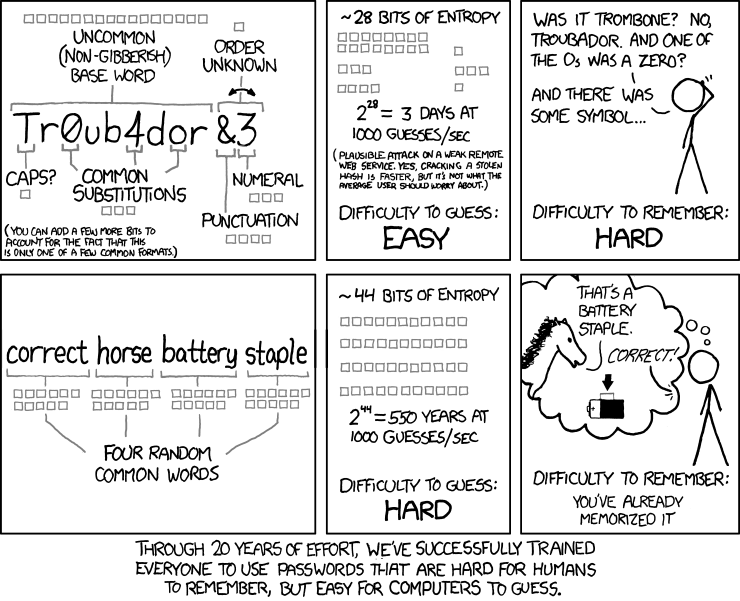
\includegraphics[width=\textwidth]{password_strength.png}

\newpage
\small
\setlength{\parindent}{0em}
\setlength{\parskip}{0.5em}

\subsubsection*{What is a Diceware passphrase?}

A passphrase is a bunch of words and characters that you type in to your computer to let it know for sure that the person typing is you. Passphrases differ from passwords only in length.

Diceware is a method for picking passphrases that uses dice to select words at random from a special list. Each word in the list is preceded by a four digit number. All the digits are between one and six, allowing you to use the outcomes of four dice rolls to select a word from the list.

\subsubsection*{Directions}

\begin{itemize}[leftmargin=*]

\item[1] Decide how many words you want in your passphrase. A four-word passphrase provides a level of security \textit{much} higher than the passwords most people use. For NSA-proof security, use seven.

\item[2] Roll all four dice at once and write the results down, reading from left to right, on a scrap paper. Make as many of these four-digit groups as you want words in your passphrase.

\item[3] Flip to the word list and look up the corresponding word next to each four-digit number.

\item[4] The words that you have found are your new passphrase! If required by an outdated password policy, capitalize a memorable word, and replace the last word with its four digit number.

\item[5] Come up with a way to remember your phrase. It might be a story, scenario, or sentence that can remind you of the phrase you generated.

\end{itemize}

\subsubsection*{Example}

Suppose you want a five-word passphrase. You will need $5 \times 4$ or 20 dice rolls. Let's say they come out as:

1, 6, 6, 6, 5, 1, 5, 6, 5, 3, 5, 6, 3, 2, 2, 3, 5, 6, 2, and 6. 

Write the results on a scrap of paper in groups of four:

1 6 6 6 \\
5 1 5 6 \\
5 3 5 6 \\
3 2 2 3 \\
5 6 2 6

You then look up each group of five rolls in the Diceware word list by finding the number in the list and writing down the word next to the number:

1666 cognitive \\
5156 poetic \\
5356 ribbon \\
3223 garlic \\
5626 smelliness

Your passphrase would then be:

cognitive poetic ribbon garlic smelliness

This passphrase is one of the 3,656,158,440,062,976 (about $2^{51}$) alternatives that could have been chosen by this method. 


\chapter*{Notes about Security}
\label{ch:qna}

\subsubsection{Shouldn't I never write my password down?}

In today's world, major corporations are hacked every week, and distributed cracking networks can break complex passwords in record time. It's safest to use a strong, unique password for each account you hold, but this makes memorization impractical. 

Once, people were told not to write passwords down, ever, but the consensus among security professionals has evolved. You're better at protecting this book than corporations are at securing their password databases. 

\subsubsection{Can I just pick my own words from the word list?}

No. Humans are terrible at being unpredictable, and hackers are great at exploiting predictability. The primary reason that Diceware creates secure passwords is that you have no agency in the process.

\subsubsection{Should I leave spaces between the words?}

Yes. It makes your passphrase more secure, \textit{and} easier to type.

\subsubsection{How many words should I use in my passphrase?}

The most important accounts, such as e-mail, e-commerce and financial sites, should use at least five words.

Encrypted drives storing sensitive personal and financial documents should use seven words.

Less important accounts, like social media, can use three words, provided each password is used only once.

\subsubsection{My passphrase was rejected because it is too long, or because it lacks capitalization and numbers.}

You may shorten words to no less than three letters without affecting the security of your passphrase, provided the shortened version remains unique within the word list. You may also replace words with their associated 4 digit number. You may \textit{not} choose different words.

Capitalization adds a very small amount of security; if required, pick a memorable word to capitalize.

\subsubsection{What if I lose this book?}

The real purpose of this book is to provide you with the tools to generate strong, memorable passwords that are unbreakable by the world's most powerful computers. It need not be the only place that you record them.

\subsubsection{Are password manager apps like 1Password safe?}

Yes, as long as the master password is strong \& secure. For example, if Google Chrome is configured to store your password, make sure that you have a strong Google password, and don't leave your account logged in on computers or mobile devices that are not physically secure. The same is true of Safari and iCloud, Internet Explorer and Windows Live, etc.

\subsubsection{Who invented Diceware?}

Diceware was invented by Arnold G. Reinhold, a computer scientist in Cambridge, MA. It was first published to Usenet's \textit{sci.crypt.research} on August \ordinalnum{1}, 1995. For lots more information, see 
\url{https://goo.gl/xobzeV}.
%\url{http://world.std.com/~reinhold/diceware.html}. 

This book implements a simplified version developed by the Electronic Frontier Foundation (EFF) in 2016, which uses only four dice.
 
\subsubsection{What is the danger in re-using a password?}

Imagine that you used the same password for an online clothing store, and your e-mail provider. Months later, the clothing store is hacked and your password is stolen. The hackers login to your email and find correspondence from your bank. They use the bank website to reset your online banking password, and intercept the confirmation email. Next, they use the bank website to order checks in your name, initiate transfers, etc.

This story illustrates why the security of your e-mail ranks above others in importance: for hackers, it is the gateway to all your accounts.

\subsubsection{How can I find out if my password has been stolen?}

Visit \url{haveibeenpwned.com}, and type in your e-mail address. They track the data leaks released by hackers, and can identify which e-mail addresses were hacked, and how much data was released.

If your e-mail tests positive, immediately change the password for the sites listed \textit{and} any sites that might have used the same password. 

\subsubsection{What is two-factor authentication?}

Two-factor authentication enhances your password by sending a code to your phone or another device, which you then have to type in order to be authorized. This ensures that even if someone has your password, they also need to have your phone.

It's a good idea to set up two-factor authentication on any account linked to your bank account or credit cards.

The US Government no longer recommends SMS for two-factor authentication, due to the ease with which text messages can be intercepted. Mobile apps such as Google Authenticator are more secure.

\subsubsection{What is phishing?}

Phishing is when a hacker sends you an email that appears to be from an organization you have a relationship with, but is actually a trap to get you to give up your password.

Phishing e-mails typically warn you that something is wrong with your account, and urge you to log in via a link. They can be very realistic and insidious.

Always check the URL in any e-mailed links you click, and make sure that they take you to the site you expect.

\subsubsection{What is social engineering?}

Social engineering is when a hacker contacts a company you do business with and pretends to be you. Often this means telling customer service that you have lost your password, and trying to convince the representative to change it or otherwise unlock your account.

The best protection against social engineering is to avoid using easily-guessed security questions, such as your mother's maiden name. When asked for such information, generate a Diceware password instead.

\subsubsection{How can I stay safe online?}

Above all, practice good operational security (\textit{opsec}). Be suspicious and careful online. 

Minimize the number of accounts you open, and always choose the best account security available. Keep track of the accounts you open, close unused accounts, and change passwords on active accounts regularly. Prefer to shop with businesses that have strong online safeguards, and take advantage of identity protection and online shopping protection services offered by reputable financial institutions.

\subsubsection{What to do if I've been hacked?}

The resources at \url{www.crashoverridenetwork.com} and \\  \url{staysafeonline.org} are a good starting point. They provide tools that help determine whether you have been hacked and can help regain control over your online accounts.


%\par\vspace{\fill}
%\large
%\ccbysa \fill \small{https://github.com/wadetb/dicebook}

\end{document}